% !TEX program = xelatex
\documentclass[UTF8,a4paper,12pt]{ctexart}
\usepackage[a4paper,margin=2.35cm,headheight=15pt]{geometry}
\usepackage{booktabs,longtable,tabularx,array}
\usepackage{xcolor,enumitem,float,listings,graphicx}
\usepackage{xurl}
\usepackage{hyperref,fancyhdr,caption}

\definecolor{codebg}{RGB}{247,248,250}
\definecolor{linkblue}{RGB}{31,78,121}
\hypersetup{
  colorlinks=true,
  linkcolor=black,
  urlcolor=linkblue,
  pdftitle={KV Database 实验报告},
  pdfauthor={胡辉宇、张文迪}
}
\lstset{
  basicstyle=\ttfamily\small,
  backgroundcolor=\color{codebg},
  frame=single,
  breaklines=true,
  columns=fullflexible,
  showstringspaces=false
}
\setlist{itemsep=0.25em,topsep=0.4em}
\setlength{\emergencystretch}{3em}
\pagestyle{fancy}
\fancyhf{}
\lhead{KV Database}
\rhead{Rust 课程大作业实验报告}
\cfoot{\thepage}
\newcommand{\code}[1]{\texttt{#1}}
\captionsetup{font=small,labelfont=bf}

\title{\textbf{KV Database}\\[0.5em]\large 基于 Rust 的教学型关系数据库系统}
\author{胡辉宇 \quad 张文迪}
\date{2026 年 7 月 18 日}

\begin{document}
\maketitle
\thispagestyle{empty}

\begin{abstract}
本文围绕 KV Database 的项目背景、系统设计、工程实现和实验验证展开。项目以 Rust 2024 为主要实现语言，从磁盘页、空闲页管理、slotted page、B+Tree、缓冲池、事务与 MVCC 开始搭建数据库内核，再向上实现 SQL 解析执行、MySQL Wire Protocol、本地 HTTP API 和 React Web 工作台，形成从 SQL 输入到磁盘持久化的完整链路。开发过程中，团队将数据库课程中的核心机制拆解为可运行、可观察、可测试的工程模块，并围绕页面边界、事务可见性、重启恢复、协议分片和演示一致性进行了多轮验证。实验结果显示，项目通过 74 个 Rust 单元/集成测试、87 项端到端协议与持久化测试，前端生产构建和数据库文件检查脚本均可复现。本文结合系统截图、命令行输出和测试结果展示主要功能，并对 SQLite、PostgreSQL、MySQL InnoDB、CMU BusTub 等参考项目的来源、借鉴点、差异和改进进行说明。
\end{abstract}

\noindent\textbf{关键词：}Rust；关系数据库；B+Tree；事务；MVCC；MySQL 协议；持久化

\tableofcontents
\newpage

\section{项目名称}

\textbf{项目名称：}KV Database——基于 Rust 的教学型关系数据库系统。

KV Database 是一个面向课程实践的关系数据库系统原型。项目在课程大作业规模内实现了客户端连接、SQL 执行、事务处理、页面存储、持久化和可视化观察等关键能力。系统采用 Cargo workspace 组织后端核心模块，并提供 MySQL TCP 接口、HTTP API 和 React Web 工作台。命令行客户端用于验证协议访问路径，图形界面用于观察表结构、索引数量、记录快照和后端执行耗时。

项目最终交付内容覆盖数据库内核、服务端、协议入口、Web 工作台、自动化测试、演示脚本和报告文档。表~\ref{tab:deliverables} 概括了最终成果。

\begin{table}[H]
\centering
\caption{项目交付物概览}
\label{tab:deliverables}
\begin{tabularx}{\textwidth}{p{3.2cm}X}
\toprule
交付物 & 说明\\
\midrule
数据库内核 & 实现页面、B+Tree、缓冲池、catalog、事务、MVCC 和 SQL 执行等核心能力。\\
协议与服务端 & 提供 MySQL Wire Protocol 入口和本地 HTTP API，支持命令行客户端与 Web 工作台复用同一执行器。\\
Web 工作台 & 提供 SQL 编辑、执行链路、执行结果、表结构、索引状态、存储记录和执行历史展示。\\
自动化测试 & 覆盖 Rust 模块测试、协议端到端测试、持久化重启测试、前端生产构建和代码质量门禁。\\
项目文档 & 包含 README、docs 项目文档、LaTeX 实验/项目报告和开源参考说明。\\
\bottomrule
\end{tabularx}
\end{table}

\section{团队成员与分工}

团队成员与主要分工见表~\ref{tab:members}。分工按照模块责任和工程贡献描述，便于与仓库结构、测试内容和演示流程对应。

\begin{table}[H]
\centering
\caption{团队成员与主要分工}
\label{tab:members}
\begin{tabularx}{\textwidth}{p{2.5cm}p{2.8cm}X}
\toprule
姓名 & 学号 & 主要负责内容\\
\midrule
胡辉宇 & 24336043 & 项目整体架构设计；存储引擎 \code{kv-storage} 开发；磁盘页、B+Tree、缓冲池和空闲页复用实现；事务管理 \code{kv-txn} 开发；MVCC 可见性与表级锁实现。\\
张文迪 & 24336155 & SQL 解析与执行 \code{kv-sql} 开发；Planner 与 Executor 实现；网络协议 \code{kv-network} 开发；HTTP API 与 Web 工作台 \code{demo-client} 实现；自动化测试、文档与实验报告整理。\\
\bottomrule
\end{tabularx}
\end{table}

\section{项目背景与目标}

\subsection{选题背景}

数据库系统是计算机系统课程中综合性较强的方向，涉及文件组织、索引结构、查询处理、事务并发、网络通信和工程化测试。成熟数据库能够稳定提供 SQL 能力，但其内部机制通常被复杂工程细节隐藏起来：一条 SQL 如何被解析为执行计划，记录如何写入固定大小页面，事务如何影响可见性，服务重启后元数据如何恢复，这些问题很难仅通过调用接口得到直观理解。因此，本项目选择实现一个规模受控的教学型关系数据库，把抽象的数据库原理落实为可以运行、调试和复现实验的代码。

选择 Rust 作为实现语言也有明确的实践意义。数据库内核涉及所有权边界、共享状态、错误传播和并发访问，Rust 的所有权模型、trait 抽象、\code{Result} 错误处理和线程安全类型能够帮助系统在不依赖垃圾回收的前提下保持较强的内存安全性。项目开发过程也把 Rust 的语言特性放入了真实系统场景中：页面缓存、事务状态、网络连接和错误返回都经过了清晰的类型设计。

\subsection{拟解决的问题}

围绕上述背景，项目主要聚焦五类核心问题：

\begin{enumerate}[label=\arabic*.]
\item \textbf{完整请求链路贯通。}实现 \code{SQL -> Lexer -> Parser -> Planner -> Executor -> Transaction -> Storage} 的完整路径，使一条 SQL 能够真实进入事务层并写入存储引擎。
\item \textbf{可持久化的数据组织。}基于 4 KiB 固定大小页面、superblock、空闲页链表、catalog 和 B+Tree，支持服务正常重启后的表结构与数据恢复。
\item \textbf{事务与并发基础。}支持 \code{BEGIN}、\code{COMMIT}、\code{ROLLBACK}，实现写缓冲、读己之写、MVCC 可见性和表级锁。
\item \textbf{多入口访问。}提供兼容常用 MySQL 客户端的 TCP 协议接口，同时提供本地 HTTP API 和 React Web 工作台，兼顾标准接口和教学演示。
\item \textbf{可复现实验验证。}通过单元测试、端到端协议测试、前端构建和数据库文件检查脚本，验证正常功能、边界输入、重启持久化和演示数据真实性。
\end{enumerate}

\subsection{项目亮点与实现证据}

本项目的亮点不在于追求生产数据库的完整功能，而在于把数据库系统中的关键概念落实到一个可运行、可检查、可复现的工程系统中。表~\ref{tab:highlights}概括了项目中最能体现工作量和设计思考的部分。

\begin{table}[H]
\centering
\caption{项目亮点与实现证据}
\label{tab:highlights}
\small
\begin{tabularx}{\textwidth}{p{3.0cm}X X}
\toprule
亮点 & 具体体现 & 证据位置\\
\midrule
端到端链路完整 & 一条 SQL 会经过词法分析、语法解析、逻辑计划、执行器、事务管理和存储引擎，最终落到 B+Tree 和磁盘页。 & \code{kv-sql}、\code{kv-txn}、\code{kv-storage}，以及端到端协议测试。\\
存储实现可解释 & 实现 superblock、空闲页链表、slotted page、B+Tree、catalog 和 LRU 缓冲池，并对损坏页、越界槽目录和空闲页环进行检查。 & \code{pager.rs}、\code{page.rs}、\code{btree.rs}、\code{buffer.rs}。\\
事务语义可观察 & 支持显式事务、提交/回滚、读己之写、写缓冲和表级锁，Web 工作台可以观察事务前后数据状态变化。 & \code{executor.rs}、\code{manager.rs}、\code{lock.rs}、Web 事务截图。\\
交付闭环完整 & 同时提供 MySQL TCP 入口、HTTP API、React 工作台、PowerShell 检查脚本、自动化测试和 LaTeX 报告，便于评审复现。 & README、docs、\code{scripts/}、测试输出截图。\\
\bottomrule
\end{tabularx}
\normalsize
\end{table}

\subsection{预期功能与完成范围}

\begin{table}[H]
\centering
\caption{预期功能与当前完成情况}
\begin{tabularx}{\textwidth}{p{2.3cm}X p{1.5cm}}
\toprule
模块 & 功能范围 & 状态\\
\midrule
SQL & \code{CREATE TABLE}、\code{DROP TABLE}、\code{CREATE INDEX}、\code{SELECT}、\code{INSERT}、\code{UPDATE}、\code{DELETE} & 完成\\
查询 & \code{WHERE} 条件过滤、投影、\code{ORDER BY} 排序、等值 \code{JOIN}、比较与逻辑表达式 & 完成\\
事务 & \code{BEGIN}、\code{COMMIT}、\code{ROLLBACK}、写缓冲、MVCC 可见性、表级锁 & 完成\\
存储 & 4 KiB 页面、Pager、slotted page、缓冲池、B+Tree、catalog、空闲页复用 & 完成\\
协议 & MySQL 握手、命令包、结果集、错误响应、TCP 分片组包与请求大小限制 & 完成\\
Web & SQL 编辑器、执行历史、结果表、schema 面板、索引状态、数据重置 & 完成\\
恢复 & 正常关闭/重启后的表结构、记录和删表状态恢复 & 完成\\
崩溃恢复 & WAL、checkpoint、崩溃原子恢复、完整死锁检测 & 未实现\\
\bottomrule
\end{tabularx}
\end{table}

\subsection{项目使用场景与完成度评价}

项目主要面向课程展示、数据库原理学习和 Rust 系统编程实践三个场景。课程展示侧重系统可运行、过程可观察；数据库原理学习侧重页面、索引、事务和持久化机制可解释；Rust 系统编程实践则侧重模块边界、错误处理和测试复现。结合这三个场景，项目完成度主要从以下方面评价：

\begin{enumerate}[label=\arabic*.]
\item Web 工作台和 MySQL 客户端均可执行 SQL，并返回真实后端结果。
\item 建表、插入、查询、更新、删除、索引、事务提交和事务回滚均可被演示和测试。
\item 服务正常重启后，表结构、记录数据和删表状态能够恢复。
\item 测试流程能够在干净环境中复现，结果由自动化脚本和终端输出支撑。
\item 报告和演示材料能够说明参考开源项目的来源、许可证、借鉴点、本项目差异和当前边界。
\end{enumerate}

\section{系统设计与实现思路}

\subsection{整体架构}

项目采用分层架构，依赖关系自上而下保持单向。MySQL 客户端和 Web 工作台是两个入口，但二者最终共享同一个 SQL 执行器、事务层和存储层。

\begin{verbatim}
MySQL CLI --> kv-network --+
                           +--> kv-sql --> kv-txn --> kv-storage --> kv.db
Web UI ----> HTTP API -----+
\end{verbatim}

\begin{table}[H]
\centering
\caption{主要模块职责}
\begin{tabularx}{\textwidth}{p{3.2cm}X}
\toprule
模块 & 职责\\
\midrule
\code{kv-common} & 跨模块共享的类型、错误定义和 \code{Pager} trait。\\
\code{kv-storage} & 页面管理、磁盘 Pager、slotted page、缓冲池、B+Tree、catalog 和存储引擎。\\
\code{kv-txn} & 事务生命周期管理、写缓冲、MVCC 可见性和表级锁。\\
\code{kv-sql} & Lexer、Parser、Planner 和 Executor，负责 SQL 语义到存储操作的转换。\\
\code{kv-network} & MySQL Wire Protocol、TCP 连接处理、分片重组和结果编码。\\
\code{kv-server} & 服务组装、本地 HTTP API、演示状态查询和重置接口。\\
\code{demo-client} & React + Vite 数据库工作台，展示 SQL、结果集、schema、索引和后端耗时。\\
\bottomrule
\end{tabularx}
\end{table}

这种结构的核心价值在于边界清晰。网络层和 HTTP 层承担协议转换，SQL 层负责语法语义和执行调度，事务层处理可见性与提交/回滚，存储层不依赖前端或网络协议。入口层复用同一套业务规则，使 MySQL 客户端、Web 工作台和自动化测试获得一致的执行结果。

\subsection{设计原则与方案取舍}

项目设计遵循三个原则。第一，\textbf{教学闭环优先}：系统从 SQL 输入一直贯通到磁盘页，协议、SQL、事务和存储层共同构成完整执行路径。第二，\textbf{可验证优先}：关键模块都配有自动化测试或脚本观察方式，例如数据库文件检查脚本可以直接读取 superblock 和 Web 状态，使实验结果具备文件级和接口级证据。第三，\textbf{复杂度受控}：当前阶段聚焦页面、B+Tree、事务语义、协议基本路径和演示可观察性，WAL、完整崩溃恢复、行级锁和完整 MySQL 兼容性作为后续扩展方向。

这些取舍体现了团队对课程项目规模的判断：项目在功能数量、实现深度和可复现性之间保持平衡，重点放在链路贯通、边界清楚和证据可复现上。

\subsection{工程实现过程与关键行动}

项目开发过程大致经历了四个阶段。第一阶段集中在存储层，团队先确定 4 KiB 固定页、superblock、空闲页链表和 slotted page 的文件组织方式，再实现 B+Tree 查找、插入、分裂和扫描。这个阶段重点处理变长记录、页内槽目录、文件格式校验、页号复用和损坏文件检测等底层问题。

第二阶段把存储能力接入事务层和 SQL 层。团队实现 Lexer、Parser、Planner、Executor，并将 \code{CREATE TABLE}、\code{INSERT}、\code{SELECT}、\code{UPDATE}、\code{DELETE} 等语句映射到 catalog、B+Tree 和事务写缓冲。事务部分加入 \code{BEGIN}、\code{COMMIT}、\code{ROLLBACK}、读己之写和 MVCC 可见性，使系统能够展示数据库课程中常见的事务语义。

第三阶段补齐外部访问入口。团队实现 MySQL Wire Protocol 的握手、命令包、结果集和错误响应，使系统可以被标准 MySQL 客户端连接；同时实现本地 HTTP API 和 React Web 工作台，将 SQL 执行链路、schema、索引数量、存储记录和执行耗时展示出来。前端通过后端 API 获取状态，不在浏览器端伪造 SQL 结果，因此界面展示与后端状态保持一致。

第四阶段围绕复现和展示进行整理。团队补充 Rust 模块测试、端到端 TCP 协议测试、重启持久化测试、前端生产构建检查和 PowerShell 演示脚本，并将使用、架构、测试和开源参考整理到 docs 文档中。这个阶段也暴露出 Windows PowerShell 与 bash 脚本兼容性、演示数据库初始状态、Web 操作后脚本读取哪个数据库文件等实际问题，最终通过清理演示数据库、统一脚本入口和增加只读检查输出来解决。

\subsection{关键数据结构}

\textbf{数据库文件与 superblock。}数据库文件由固定 4096 字节页面组成，page 0 是 superblock，保存 \code{next\_page\_id}、\code{free\_list\_head}、\code{catalog\_root}、\code{KVDBPAGE} 魔数和格式版本。打开文件时会检查文件长度、魔数、版本、页号范围和空闲链表环，使损坏文件能够以明确错误返回。

\begin{table}[H]
\centering
\caption{superblock 关键字段}
\begin{tabularx}{\textwidth}{p{2.5cm}p{3.4cm}X}
\toprule
偏移 & 字段 & 作用\\
\midrule
0--7 & \code{next\_page\_id} & 下一个可分配页面编号。\\
8--15 & \code{free\_list\_head} & 空闲页单链表头，用于释放页复用。\\
16--23 & \code{catalog\_root} & catalog B+Tree 根页，保存表元数据入口。\\
24--31 & \code{KVDBPAGE} & 文件格式魔数，用于拒绝错误文件类型。\\
32--35 & \code{version} & 文件格式版本，当前版本为 1。\\
\bottomrule
\end{tabularx}
\end{table}

\textbf{Slotted Page。}页面内部采用槽目录组织变长 tuple。页头保存 page id、tuple 数量、\code{free\_start}、\code{free\_end} 和标志位；槽目录记录 tuple 偏移与长度；tuple 数据区从页面另一端增长。实现中的 \code{validate\_layout} 会检查槽目录边界、tuple 范围和重叠关系，使损坏数据以显式错误返回。

\textbf{B+Tree。}B+Tree 内部节点保存分隔键和子页号，叶节点保存有序键值并通过 \code{next} 形成叶链。插入时先沿分隔键定位叶页，再按序插入；节点超容量时分裂并向父节点上推分隔键；根节点分裂时创建新根。叶链支持范围扫描和顺序遍历。当前删除路径覆盖基本删除，但尚未实现完整合并和再平衡。

\textbf{缓冲池。}项目使用 Rust \code{Pager} trait 抽象页面读写、分配、释放和刷盘，并通过 \code{BufferedPager} 包装磁盘 Pager。缓冲池使用 \code{Mutex} 保护 LRU 状态；释放页面时显式删除缓存副本，保证页号复用后读取到的是新页面内容。

\subsection{核心算法与实现流程}

\textbf{SQL 执行流程。}SQL 字符串先进入 Lexer 生成 token，再由 Parser 构建语法树，Planner 生成执行计划，Executor 根据计划调用事务层与存储层。对于写操作，执行器先进入事务写缓冲，提交时落盘，回滚时丢弃；对于读操作，执行器结合事务可见性规则读取当前会话可见版本。

\textbf{MVCC 与表级锁。}事务层维护事务状态、写集和版本可见性，使同一事务内可以读到自己尚未提交的写入，即 read-your-writes。当前锁粒度为表级锁，覆盖演示所需的并发安全基础；行级锁和死锁图属于后续可扩展方向。

\textbf{页面分配与回收。}分配新页面时优先从 \code{free\_list\_head} 指向的空闲页链表取页，若无空闲页则使用 \code{next\_page\_id} 扩展文件。释放页面时将其写入空闲链表。测试覆盖了重启后的页面复用和空闲链表环检测。

\textbf{协议与展示。}MySQL 服务实现握手、命令包、OK/ERR 包和结果集编码，并支持 TCP 分片组包。HTTP API 提供 \code{GET /api/state}、\code{POST /api/query}、\code{POST /api/reset}，请求体上限为 64 KiB。React 工作台通过后端 API 获取状态，不在前端复制 SQL 或事务规则，因此展示结果来自真实后端状态。

\subsection{关键代码位置}

\begin{longtable}{>{\raggedright\arraybackslash}p{0.46\textwidth}>{\raggedright\arraybackslash}p{0.46\textwidth}}
\caption{关键实现文件}\\
\toprule
文件 & 主要实现\\
\midrule
\endfirsthead
\toprule
文件 & 主要实现\\
\midrule
\endhead
\code{crates/kv-storage/src/pager.rs} & 数据库文件格式、superblock、空闲页链表、文件打开校验和刷盘。\\
\code{crates/kv-storage/src/page.rs} & Slotted Page 编解码、槽目录、tuple 边界验证。\\
\code{crates/kv-storage/src/btree.rs} & B+Tree 查找、插入、分裂、删除和扫描。\\
\code{crates/kv-storage/src/buffer.rs} & LRU 缓冲池、页面缓存和释放页缓存失效。\\
\code{crates/kv-txn/src/} & 事务状态机、MVCC、写缓冲和表级锁。\\
\code{crates/kv-sql/src/} & 词法分析、语法分析、计划生成和 SQL 执行。\\
\code{crates/kv-network/src/protocol.rs} & MySQL 包解析、结果编码、分片与错误响应。\\
\code{crates/kv-server/src/demo\_http.rs} & HTTP 路由、状态快照、查询执行和重置接口。\\
\code{demo-client/src/App.jsx} & Web 工作台状态、执行历史、schema 与结果展示。\\
\bottomrule
\end{longtable}

\section{实验结果}

\subsection{实验环境与复现方法}

实验在 Windows 环境下进行，使用 Rust/Cargo、Node.js/npm 和 Python 脚本完成验证。核心复现命令如下：

\begin{lstlisting}[language=bash]
cargo fmt --check --all
cargo clippy --workspace --all-targets -- -D warnings
cargo test --workspace --all-targets
cargo doc --workspace --no-deps

cd demo-client
npm ci
npm run build
cd ..

python test_protocol.py
git diff --check
\end{lstlisting}

仓库还提供 \code{scripts/run-and-show-tests.ps1}，将上述质量门禁整理为提交核验用的终端摘要；\code{scripts/show-kv-db.ps1} 以只读方式解析数据库文件页信息，并在服务运行时读取 Web API 当前表数据，用于交叉验证 Web 操作、后端状态和数据库文件之间的对应关系。

\subsection{已实现功能总览}

\begin{table}[H]
\centering
\caption{功能验证结果}
\begin{tabularx}{\textwidth}{p{3.1cm}X p{1.6cm}}
\toprule
实验项 & 实际结果 & 结论\\
\midrule
SQL DDL/DML & 建表、删表、建索引、插入、更新、删除和查询均可执行。 & 通过\\
查询能力 & 条件过滤、投影、排序、等值 JOIN、比较和逻辑表达式均有测试覆盖。 & 通过\\
事务语义 & \code{BEGIN/COMMIT/ROLLBACK}、事务内读己之写、回滚恢复均通过。 & 通过\\
持久化 & 正常重启后表结构、记录数据、已删表状态均可恢复。 & 通过\\
协议接口 & MySQL 握手、命令包、结果集、错误包、TCP 分片和截断输入均可处理。 & 通过\\
Web 工作台 & 可执行 SQL、查看结果集、schema、索引数量、记录数量和后端执行耗时。 & 通过\\
\bottomrule
\end{tabularx}
\end{table}

\subsection{项目界面与功能展示}

项目成果既体现在后端模块中，也体现在最终系统的使用方式中。图~\ref{fig:web-index} 展示 Web 工作台的核心界面：左侧是项目模板与执行历史，中间是 SQL 编辑器和执行结果，右侧展示 SQL 从词法、语法、计划、事务、B+Tree 到结果集的执行链路，下方展示真实后端返回的数据表状态和存储记录。该界面把数据库内部执行过程转化为可观察的项目成果，使课程演示和调试过程更加直观。

\begin{figure}[H]
\centering
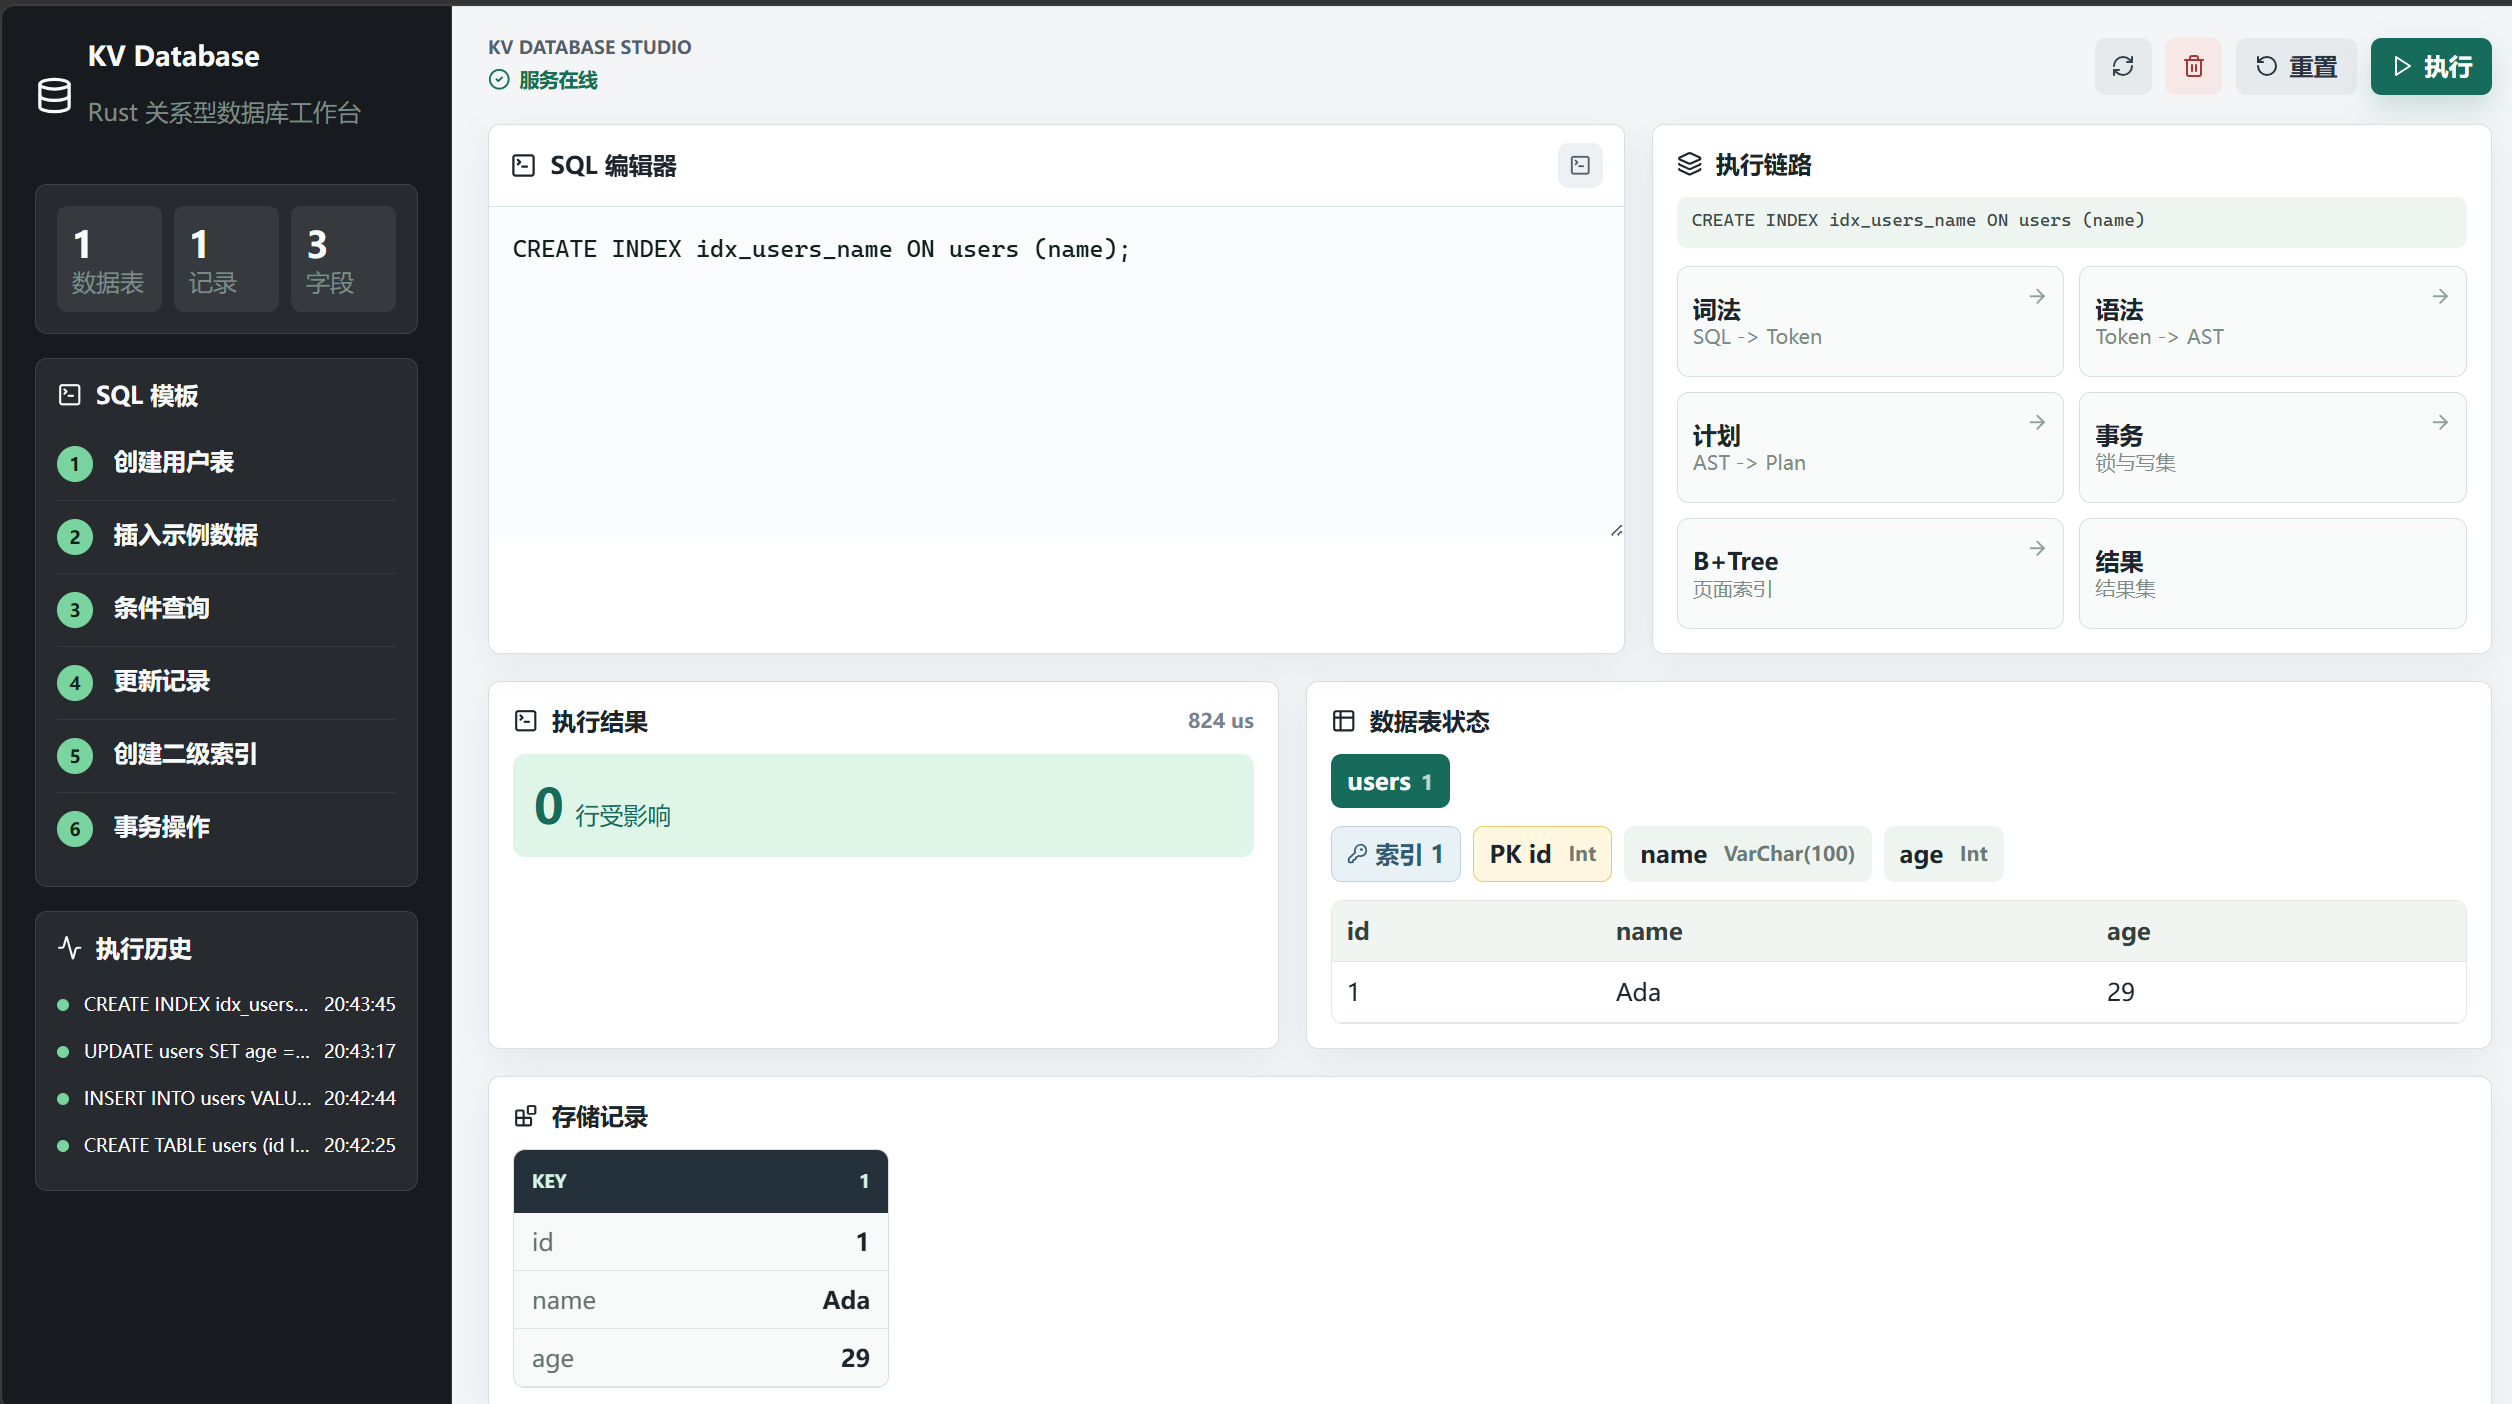
\includegraphics[width=\textwidth]{figures/web-index-state.png}
\caption{Web 工作台中的二级索引创建与数据表状态展示}
\label{fig:web-index}
\end{figure}

图~\ref{fig:web-transaction} 展示事务场景。工作台执行 \code{BEGIN}、\code{INSERT}、\code{UPDATE}、\code{SELECT}、\code{COMMIT} 后，右侧表状态显示 Grace 记录已经提交，执行链路中同时标出事务、B+Tree 和结果集阶段。这个过程体现了前后端边界的处理方式：前端负责展示和交互，状态变化由 HTTP API 调用后端 SQL 执行器完成，再由事务层和存储层共同落到系统状态中。

\begin{figure}[H]
\centering
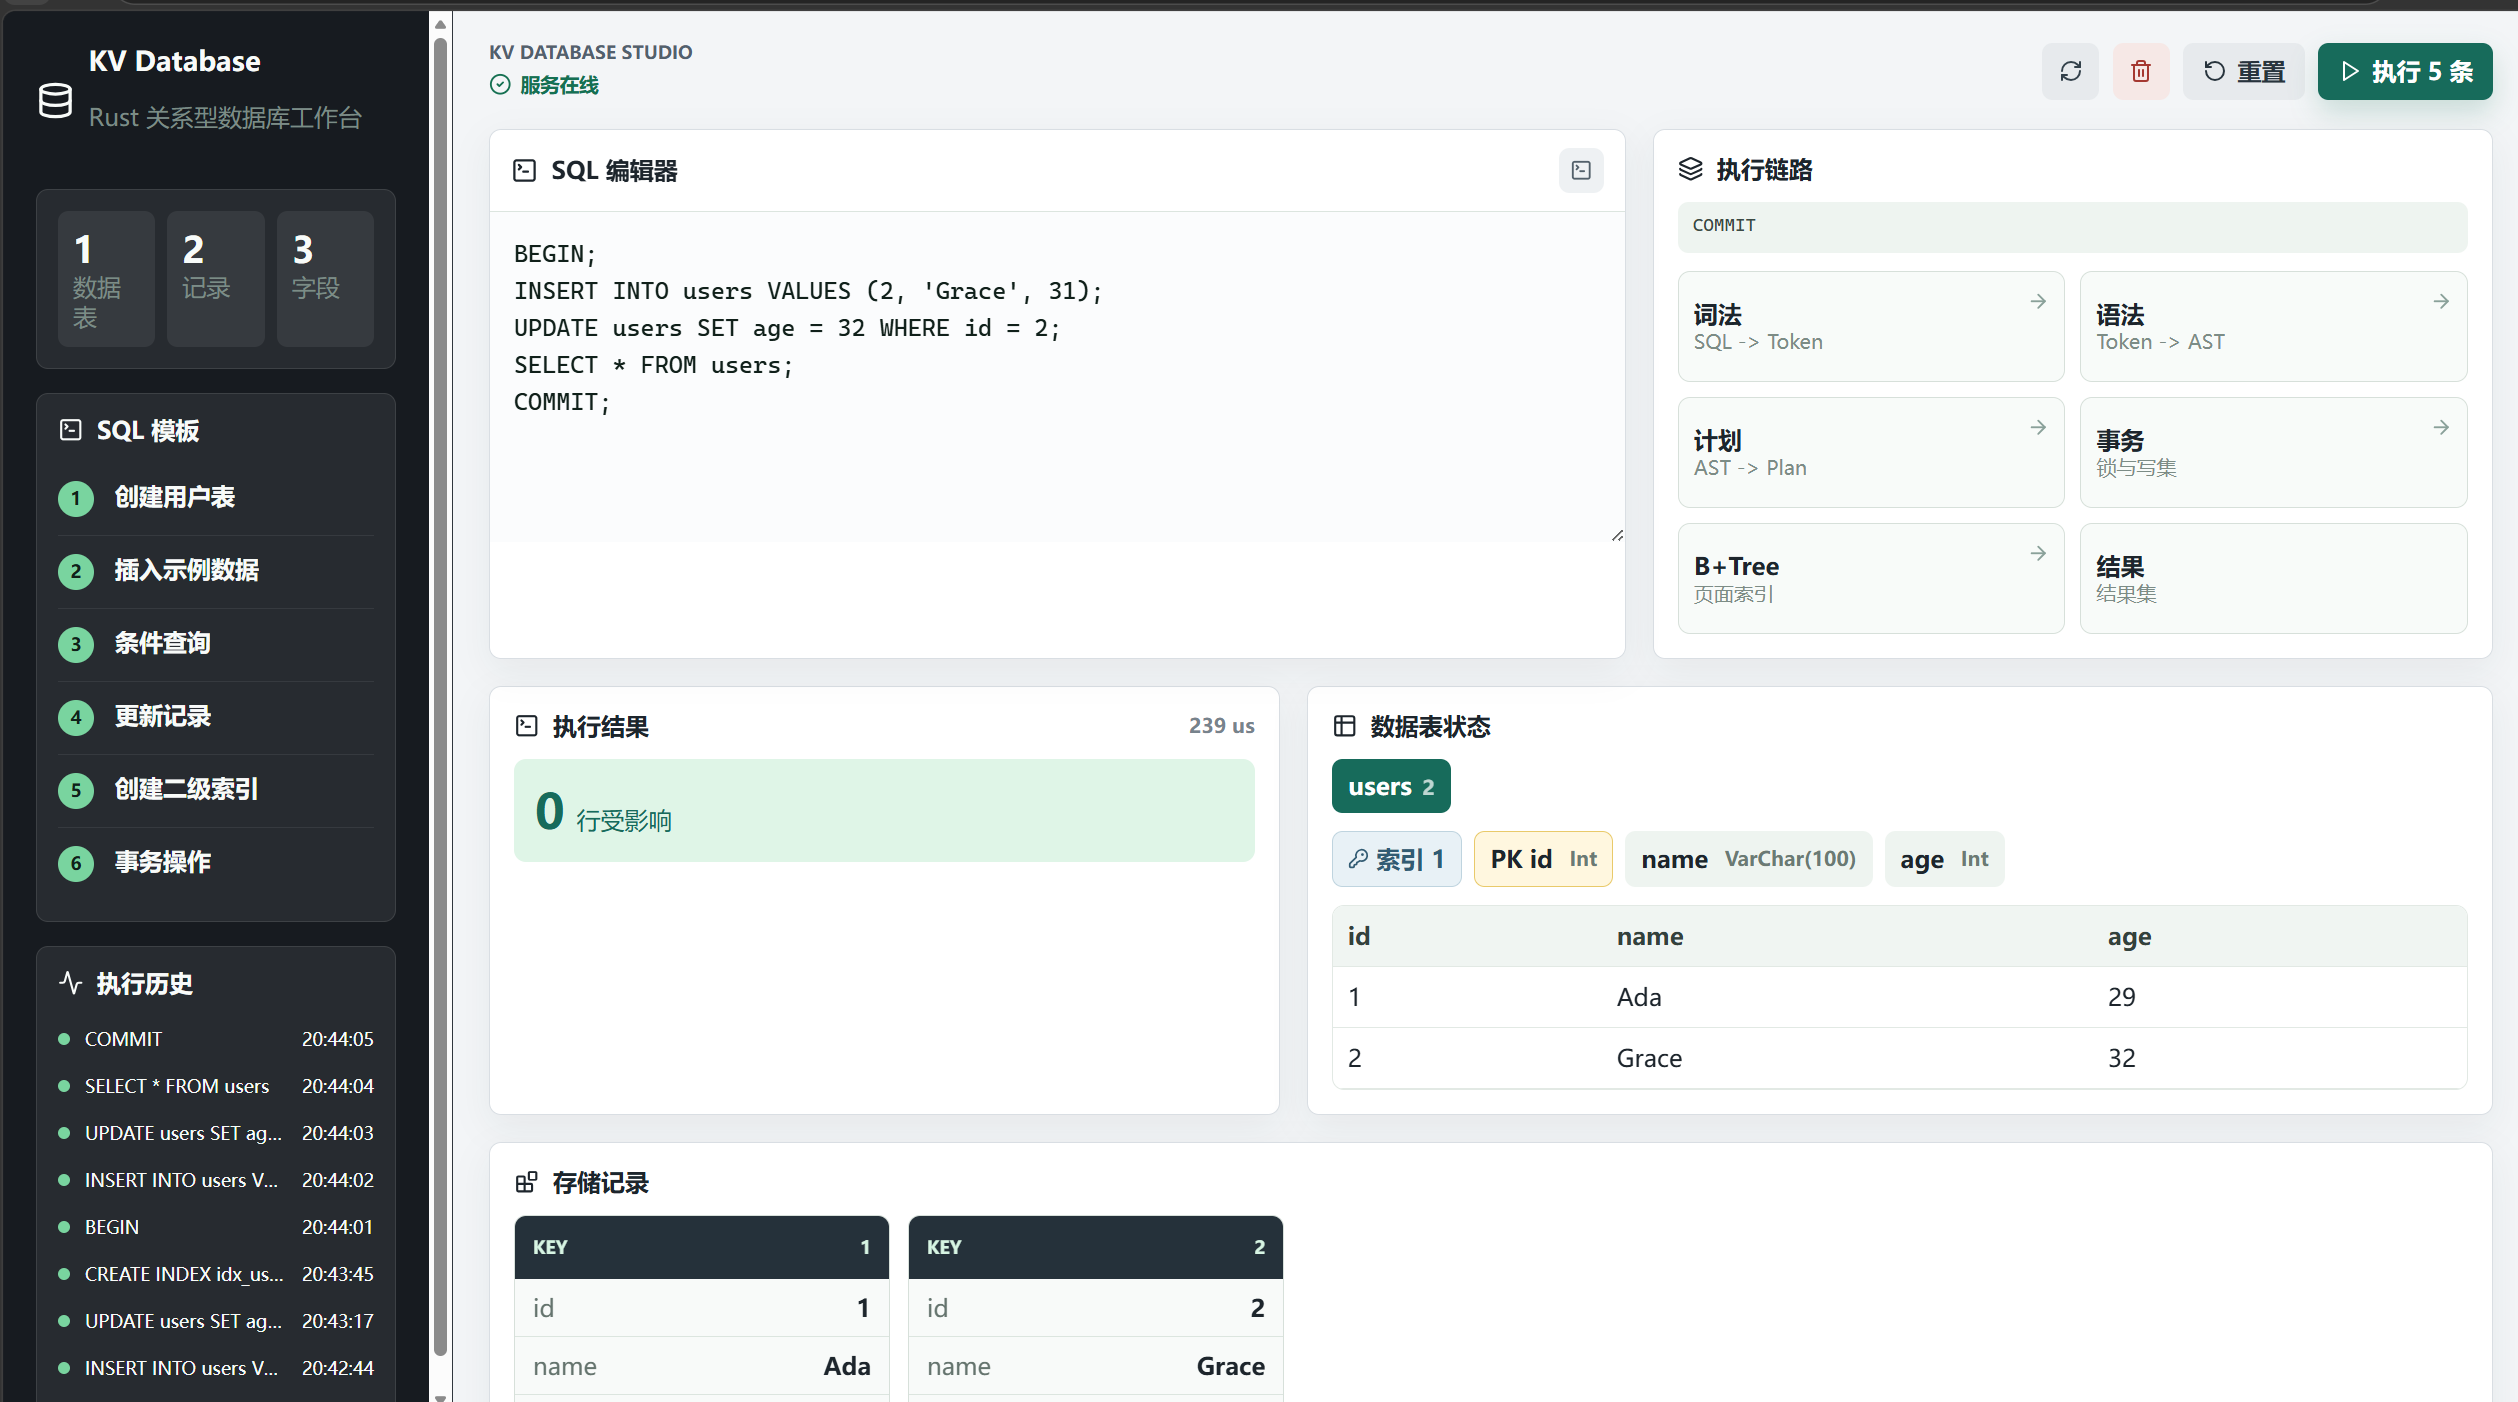
\includegraphics[width=\textwidth]{figures/web-transaction.png}
\caption{Web 工作台中的事务提交与记录状态展示}
\label{fig:web-transaction}
\end{figure}

\subsection{测试结果与证据}

当前项目包含两层主要测试证据。第一层是 Rust workspace 内的单元测试和集成测试，共 74 项，覆盖共享类型、网络协议、服务端、SQL、存储和事务模块。第二层是 \code{test\_protocol.py} 端到端协议/持久化测试，共 87 项，通过真实 TCP 连接验证 SQL、事务、索引、错误处理和服务重启。两层测试分别覆盖模块内部正确性和系统级可用性，使项目评价同时具备模块级证据和系统级证据。

\begin{table}[H]
\centering
\caption{自动化测试结果汇总}
\begin{tabularx}{\textwidth}{p{3.2cm}X p{1.6cm}}
\toprule
测试类别 & 覆盖内容与结果 & 结论\\
\midrule
Rust 测试 & 8 个测试目标共 74 项，74 项通过，0 失败。 & 通过\\
协议测试 & MySQL TCP、DDL/DML、JOIN、事务、错误输入和持久化恢复共 87 项，87 项通过。 & 通过\\
前端构建 & React/Vite 生产构建成功，可生成可部署静态资源。 & 通过\\
质量门禁 & 格式检查、Clippy、文档生成和空白差异检查均纳入提交前流程。 & 通过\\
\bottomrule
\end{tabularx}
\end{table}

端到端脚本的关键输出如下：

\begin{lstlisting}
[31] PASS JOIN ... ON table.col = table.col
[46] PASS Row visible inside txn (write buffer)
[57] PASS ROLLBACK (undo DELETE)
[85] PASS After restart: data + metadata persisted
[87] PASS After restart: dropped table stays dropped
Total: 87, 87 passed
\end{lstlisting}

数据库文件检查脚本可展示文件级证据和 Web 操作后的真实状态。例如在 Web 工作台执行建表和插入后，脚本会输出 \code{KVDBPAGE}、页大小、catalog root，并列出当前 \code{users} 表的字段与记录。图~\ref{fig:db-inspection} 是对应终端证据。

\begin{lstlisting}
KV database file inspection (read-only)
page size:        4096 bytes
superblock magic: KVDBPAGE
catalog root:     1

Web state from kv-server
table count:      1
row count:        3
table:            users
columns:          id, name, age
data:
  id | name | age
  1 | Ada | 28
  2 | Grace | 31
  3 | Linus | 25
\end{lstlisting}

\begin{figure}[H]
\centering
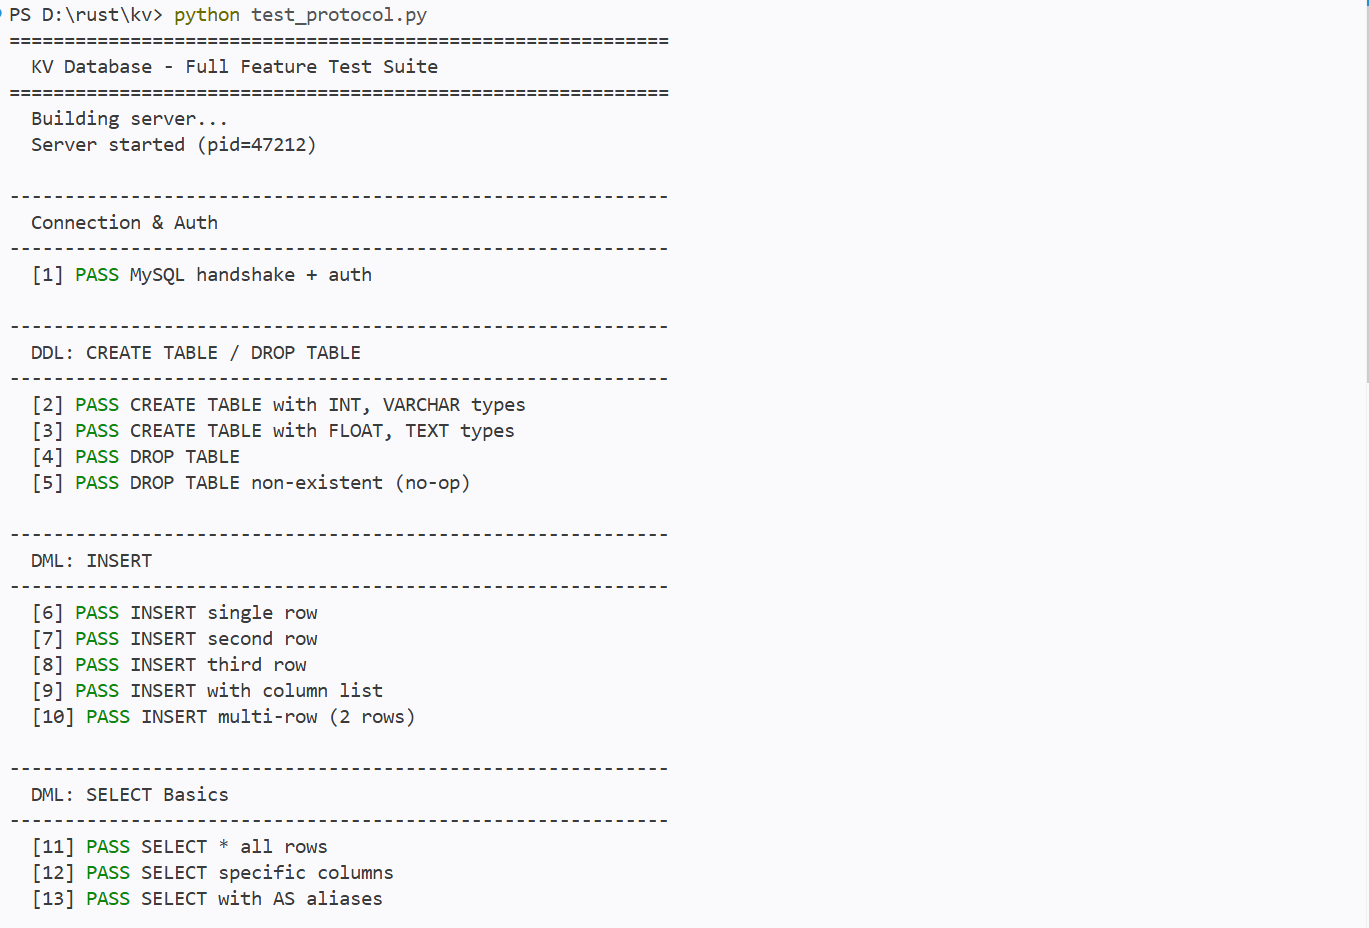
\includegraphics[width=0.92\textwidth]{figures/db-file-inspection.png}
\caption{数据库文件页信息与 Web 状态检查结果}
\label{fig:db-inspection}
\end{figure}

协议测试进一步覆盖错误输入、删表重建和重启持久化等系统级场景。图~\ref{fig:persistence-tests} 显示端到端测试最后阶段：错误处理、DROP TABLE 后重建、数据与元数据跨重启恢复、删表状态跨重启保持均通过，最终结果为 \code{Total: 87, 87 passed}。

\begin{figure}[H]
\centering
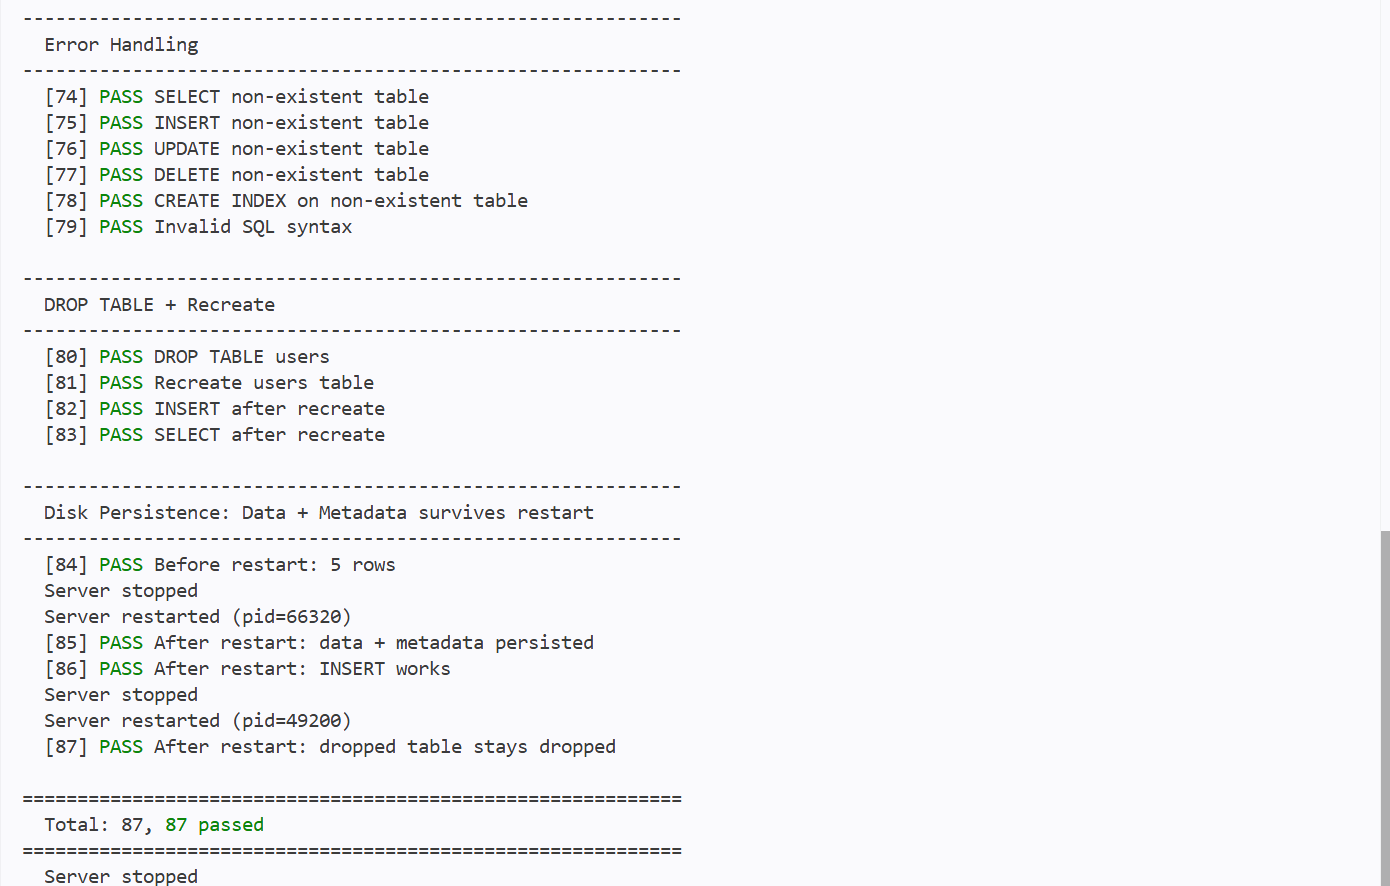
\includegraphics[width=0.92\textwidth]{figures/protocol-persistence-tests.png}
\caption{端到端协议与持久化测试结果}
\label{fig:persistence-tests}
\end{figure}

\subsection{运行示例}

启动后端服务：

\begin{lstlisting}[language=bash]
cargo run -p kv-server
\end{lstlisting}

默认监听地址为：MySQL Wire Protocol \code{127.0.0.1:3307}，演示 HTTP API \code{127.0.0.1:8080}，数据文件 \code{./kv\_data/kv.db}。使用 MySQL 客户端连接：

\begin{lstlisting}[language=bash]
mysql -h 127.0.0.1 -P 3307 -u root
\end{lstlisting}

示例 SQL：

\begin{lstlisting}[language=SQL]
CREATE TABLE users (id INT PRIMARY KEY, name VARCHAR(100), age INT);
INSERT INTO users VALUES (1, 'Ada', 28), (2, 'Grace', 31);
SELECT id, name FROM users WHERE age > 28 ORDER BY id;
BEGIN;
UPDATE users SET age = 32 WHERE id = 2;
ROLLBACK;
\end{lstlisting}

启动 Web 工作台：

\begin{lstlisting}[language=bash]
cd demo-client
npm ci
npm run dev
\end{lstlisting}

访问 \url{http://127.0.0.1:5173} 后即可通过图形界面执行 SQL，并观察 schema、索引、记录和执行耗时。

\subsection{结果分析与局限}

实验结果表明，项目已经形成从 SQL 输入、协议解析、事务执行、B+Tree 存储到磁盘持久化的最小闭环。端到端测试和数据库文件检查脚本分别提供系统级和文件级证据：前者证明系统能够通过真实 TCP 连接执行功能并跨重启恢复，后者证明 Web 操作后的状态可以从后端 API 和数据库文件层面同时观察。由此可以判断，项目成果由后端执行链路、存储格式、Web 工作台和验证脚本共同构成。

同时，项目边界也保持清晰。当前版本的恢复能力以正常关闭和重启后的持久化为主，尚未覆盖 WAL、崩溃原子恢复、完整 B+Tree 删除再平衡、完整 MVCC 版本链、行级锁、死锁检测、用户认证和完整 MySQL 兼容性。因此本实验结论限定为：在课程项目设计范围内，系统功能较完整、测试可复现、边界处理明确；项目定位为教学型数据库系统原型。

\section{开源项目参考说明}

\subsection{参考来源与引用方式}

本项目在设计阶段查阅了多个成熟开源数据库和教学数据库项目的公开资料。参考重点不是复制具体源码，而是理解数据库系统中已经被反复验证的设计边界：数据库文件如何标识和管理空闲页，数据页如何组织变长记录，B+Tree 如何支持索引和范围访问，缓冲池如何隔离上层逻辑与页面读写。项目代码采用独立实现，引用材料在 README、docs 文档和本报告中列出，并标明参考对象、许可证、参考内容以及本项目对应实现文件。主要参考来源见表~\ref{tab:opensource}，对应实现主要位于 \code{pager.rs}、\code{page.rs}、\code{btree.rs}、\code{buffer.rs} 和 \code{traits.rs}。

\begin{table}[H]
\centering
\caption{开源项目参考来源}
\label{tab:opensource}
\small
\begin{tabularx}{\textwidth}{p{3.0cm}p{3.1cm}X}
\toprule
参考项目 & 版本/许可证 & 参考重点\\
\midrule
SQLite & 3.50.4 源码标签；Public Domain & 参考数据库文件格式、固定大小页面、文件头信息和 free-list 管理思想。\\
PostgreSQL & REL\_18\_0 源码标签；PostgreSQL License & 参考 slotted page 的页头、line pointer/槽目录和 tuple 数据区分离思想。\\
MySQL InnoDB & mysql-8.4.0 源码标签；GPLv2 & 参考 InnoDB 以 B+Tree 组织聚簇索引和二级索引的总体结构，以及叶子层有序访问的设计思想。\\
CMU BusTub & f0d9e375 提交；MIT & 参考教学数据库的模块拆分、BufferPoolManager 职责和面向测试的工程组织。\\
\bottomrule
\end{tabularx}
\normalsize
\end{table}

主要公开链接如下：

\begin{enumerate}[label={[\arabic*]},leftmargin=2.5em]
\item SQLite Database File Format：\url{https://www.sqlite.org/fileformat2.html}
\item SQLite \code{src/btree.c}：\url{https://github.com/sqlite/sqlite/blob/version-3.50.4/src/btree.c}
\item PostgreSQL Database Page Layout：\url{https://www.postgresql.org/docs/current/storage-page-layout.html}
\item PostgreSQL \code{bufpage.h}：\url{https://github.com/postgres/postgres/blob/REL_18_0/src/include/storage/bufpage.h}
\item MySQL InnoDB Index Types：\url{https://dev.mysql.com/doc/refman/8.4/en/innodb-index-types.html}
\item MySQL \code{page0types.h}：\url{https://github.com/mysql/mysql-server/blob/mysql-8.4.0/storage/innobase/include/page0types.h}
\item CMU BusTub：\url{https://github.com/cmu-db/bustub/tree/f0d9e3753482d45f2b5919da1873684600b48508}
\end{enumerate}

\subsection{与参考项目的区别、修改和改进}

本项目对开源项目的借鉴主要体现在结构和机制层面，而不是功能规模层面的横向竞争。SQLite、PostgreSQL 和 InnoDB 都是生产级数据库系统，覆盖 WAL、恢复、并发控制、查询优化、权限和生态兼容等大量能力；BusTub 则是面向数据库课程的教学系统。KV Database 的定位介于“课程实现”和“完整工程交付”之间：保留数据库内核中最关键、最可解释的路径，同时把协议入口、Web 可观察性和复现实验脚本纳入交付范围。具体差异见表~\ref{tab:opensource-compare}。

\begin{table}[H]
\centering
\caption{参考系统与本项目的对比分析}
\label{tab:opensource-compare}
\small
\begin{tabularx}{\textwidth}{p{2.3cm}p{4.25cm}X}
\toprule
维度 & 参考系统做法 & 本项目取舍与对应实现\\
\midrule
文件与空闲页 & SQLite 文件格式以固定页面为基础，维护数据库头部信息，并使用 free-list trunk/leaf 管理空闲页；生产环境还配合 journal 或 WAL 保证恢复语义。 & 本项目实现独立 superblock，保存魔数、格式版本、下一页号、空闲链表头和 catalog 根页。空闲页用页内前 8 字节串成单链表，便于课程规模下说明页号复用；同时增加截断文件、非法页号和 free-list 环检测。\\
数据页 & PostgreSQL 页面布局使用页头、item identifier/line pointer、tuple 数据区和 special space，并为 WAL、校验、剪枝等机制保留字段。 & 本项目实现精简 slotted page：页头记录页号、槽数量和空闲区边界，槽目录向后增长，tuple 数据从页尾向前增长。实现重点放在变长记录组织和损坏页面校验，而不是复制 PostgreSQL 的 WAL 与 vacuum 相关字段。\\
索引结构 & InnoDB 以 B+Tree 组织聚簇索引和二级索引，索引页还涉及页目录、记录头、页分裂、并发访问、redo/undo 恢复等生产级机制。 & 本项目实现固定阶 B+Tree，包含内部节点、叶节点、节点分裂、根节点更新和叶子链范围扫描。为了保证实现可读和测试稳定，暂不实现复杂删除再平衡、页压缩和崩溃恢复。\\
缓冲池 & BusTub 将磁盘管理、BufferPoolManager、页面保护和替换策略分层，适合教学环境中逐步实现并测试。 & 本项目将页面接口抽象为 \code{Pager} trait，并在其外层实现写穿式 LRU 缓存。释放页时主动失效缓存，避免页号复用后读到旧页内容；该行为有专门测试覆盖。\\
工程入口 & SQLite、PostgreSQL、InnoDB 更关注成熟客户端生态和生产功能；BusTub 更关注课程实验框架与单元测试。 & 本项目把内核实现、MySQL Wire Protocol、HTTP API、React 工作台、PowerShell 脚本和报告文档放在同一交付闭环中。评审者既可以用标准客户端执行 SQL，也可以通过 Web 和脚本观察后端真实状态。\\
\bottomrule
\end{tabularx}
\normalsize
\end{table}

\subsection{参考后的项目特色}

通过对比可以看出，本项目主要吸收公开系统中的数据结构、模块边界和工程经验，并结合课程目标形成了以下特色：

\begin{enumerate}[label=\arabic*.]
\item \textbf{独立实现而非封装现成数据库。}项目没有调用 SQLite、PostgreSQL 或 MySQL 作为底层引擎，SQL 执行、事务缓冲、B+Tree、页面文件和协议结果编码均由项目代码完成。
\item \textbf{核心机制压缩到可解释规模。}项目保留数据库系统最重要的路径：SQL 到逻辑计划、事务状态、主键编码、B+Tree 查找/扫描、页面分配和磁盘持久化，使报告和代码能够对应解释。
\item \textbf{边界检查体现工程意识。}文件格式魔数、版本号、页号范围、free-list 环、槽目录越界、B+Tree 页面截断、TCP 分片、HTTP 请求大小和缓存失效均有处理或测试，不只验证正常输入。
\item \textbf{观察方式服务课程评审。}MySQL 协议用于标准客户端验证，Web 工作台用于展示 schema、记录和耗时，数据库检查脚本用于读取文件级信息，三者共同证明数据来自真实后端。
\item \textbf{边界说明清楚。}报告明确说明 WAL、崩溃原子恢复、完整删除再平衡、持久化 MVCC 版本链、行级锁、死锁检测和完整 MySQL 兼容性尚未实现，避免把教学原型描述成生产数据库。
\end{enumerate}

因此，本项目相对于参考项目的价值不在于功能规模，而在于把数据库系统的关键机制压缩成一个能够运行、测试、观察和解释的工程闭环。它既能体现对成熟数据库设计的理解，也能通过独立代码、测试结果和界面展示证明课程范围内的实现质量。

\end{document}
